%!TEX root = ../thesis.tex
%*******************************************************************************
%****************************** Third Chapter **********************************
%*******************************************************************************
\chapter{Discussion}

% **************************** Define Graphics Path **************************
\ifpdf
    \graphicspath{{Chapter4/Figs/Raster/}{Chapter4/Figs/PDF/}{Chapter4/Figs/}}
\else
    \graphicspath{{Chapter4/Figs/Vector/}{Chapter4/Figs/}}
\fi

\section{Summary of findings}

In chapter 2, I hypothesise that CCS bases are, in fact, the most accurate among commercially available sequencing platforms, and I develop a tool, himut, to leverage CCS read length and base accuracy for single molecule somatic mutation detection. I benchmark himut’s performance using samples where each sample has a distinct somatic mutational process and where a single somatic mutational process is responsible for newly acquired somatic mutations. The introduction of himut enables researchers to call somatic mutations, in addition to germline mutation and base modification detection from a single human genome using a single SMRTcell and the Revio sequencing instrument. 

In chapter 3, I use CCS reads and high-quality reference from a range of eukaryotic species from the DToL project to study somatic mutagenesis across the tree of life. Until recently, our understanding of somatic mutational processes has been limited to species where high-quality reference genomes are available such as \textit{H. sapiens} and model organisms such as \textit{C. elegans} \cite{Meier2014-do} and \textit{M. musculus} \cite{Riva2020-nq}. 

To confirm that himut is applicable in non-human samples, I called somatic mutations and calculated the mutation burden of \textit{P. lineatus} samples of various ages (3, 5 and 15). The mutation burden per cell increased with age in a clock-like fashion at a rate of 40 substitutions per cell per year, demonstrating that himut is applicable in non-human samples. 

Thereafter, I use himut to detect somatic mutations in approximately 600 eukaryotic species from the DToL project. I discovered XX number of mutational signatures where SBS1-like mutational signatures were previously reported through mutational signature analysis of somatic mutations in cancers \cite{Alexandrov2020-ys} and where X number of mutational signatures (SBSX1,SBSX2, SBSX3) were new mutational signatures with an unknown aetiology.

Our analysis suggests that the emergence of a new somatic mutational process is an episodic event and once established, these processes are often conserved across species. The ubiquitous presence of the SBS1 mutational signature across the animal (annelid, bird, fish and mammal), fungi and plant (dicot) kingdom, at the earliest branching of the eukaryotic phylogenetic tree, suggests that cytosine methylation in CG dinucleotide sequence context and subsequent deamination of 5mC to thymine is an ancient process that dates back to the last eukaryotic common ancestor (LECA) or that this somatic mutational process has evolved independently in multiple eukaryotic lineages. The fact that 5mC occurs at CG, CHG and CHH sequence context in plant kingdom where H can be A, C or T nucleotides \cite{Henderson2007-mm} and that 5mC occurs in CG dinucleotides in both animal and fungi kingdom \cite{Bewick2019-tu} corroborates the former theory. 

Germline mutation is the product of somatic mutations in germ cells and inheritance of these \textit{de novo} mutations from one generation to the next before and after speciation. As the ancestral allele of germline mutation cannot be determined without sequence alignment with outgroup species, germline mutational processes often cannot be determined without \textit{de novo} mutation detection through trio-sequencing. I, however, was able to use the newly extracted somatic mutational signatures to determine the germline mutational process in each species and the relative contribution of each germline mutational process in shaping the sequence context. In addition, the high similarity between the germline and somatic mutational processes suggests that the observed somatic mutational processes are clock-like mutational processes where the mutation burden increases with the age of the sample. 

\section{Limitations}

\subsection{CCS library, sequencing and software errors}

CCS library preparation, sequencing and consensus sequence generation algorithm is currently not optimised to produce CCS reads where CCS bases are assigned the correct base-specific error probabilities. I limited the analysis to Q93 CCS bases as library errors and sequencing errors are unlikely to create substitution errors on both strands of the DNA and for these errors to be propagated to all the subreads during SMRT sequencing. The experimental design, hence, restricts the analysis of errors to cases where error probabilities of Q93 CCS bases are inaccurate or to rare cases where the combination of library and sequencing errors are pervasive in CCS reads and underlying subreads.

In chapter 2, I assess Q93 CCS base accuracy using CCS reads from normal cord blood granulocytes where few somatic mutations are present. I empirically estimate that Q93 CCS base substitution error rate ranges from Q60 to Q90 depending on the substitution and the trinucleotide sequence context. In addition, I show that false positive substitutions are derived from inaccurate base accuracy estimates. What deserves the most attention is that accurate $\sim$Q90 CCS bases can be produced for all trinucleotide sequence contexts if there are enough subreads and if correct error probabilities for subread bases are used for consensus sequence generation. 

In chapter 3, I observed a somatic mutational spectrum from several species where 1) the number of called somatic mutations were greater than that from germline mutations, 2) the somatic mutational spectrum was noticeably different from the germline mutational spectrum, and finally 3) the somatic mutation spectrum was shared between phylogenetically unrelated species. In this PhD thesis, I do not investigate the origin of this somatic mutational spectrum or the downstream consequences to germline mutation detection and to assembly quality, but I hypothesise library errors to be the primary source of this erroneous somatic mutational spectrum as CCS library preparation is the only common factor in all the samples exhibiting this issue. 

\subsection{Single-molecule somatic mutation detection}

In contrast to single-molecule resolution somatic mutation detection using duplex reads from the nanorate sequencing protocol, himut cannot ascertain at all trinucleotide sequence contexts whether an individual substitution, where a single read supports the mismatch between the read and the reference genome, is an error or a somatic mutation. In a clinical setting, where himut might be used to detect the earliest transformation of a normal tissue to a neoplastic tissue or to monitor tumour regression and relapse after treatment, the accuracy of every somatic mutation call is critical in helping the clinician arrive at the correct clinical interpretation. Any false-positive or false-negative mutation call could have serious consequences for the patient’s treatment and prognosis. 
 
Multiple mutational processes act on the genome at any given time and they can generate the same sequence-context specific mutation. Given a catalogue of somatic mutations from multiple samples, mutational signature analysis identifies the mutational signature in each sample and the contribution of each mutational signature to the mutation burden of the sample (eq. \ref{eq:1}). Each mutational signature represents the probability that a specific somatic mutational process will produce a somatic mutation in a specific sequence context. 

\begin{align}
\begin{split} 
M &\approx PE \label{eq:1} \\
\begin{bmatrix}
    m^{1}_{1} & \dots & m^{1}_{j} \\
    \vdots & \ddots & \vdots \\
    m^{96}_{1} & \dots & m^{96}_{j} \\
\end{bmatrix} &\approx
\begin{bmatrix}
    p^{1}_{1} & \dots & p^{1}_{s} \\
    \vdots & \ddots & \vdots \\
    p^{96}_{1} & \dots & p^{96}_{s} \\
\end{bmatrix} \times
\begin{bmatrix}
    e^{1}_{1} & \dots & e^{s}_{j} \\
    \vdots & \ddots & \vdots \\
    e^{s}_{1} & \dots & e^{s}_{j} \\
\end{bmatrix} 
\end{split}
\end{align}

where $M$ is the somatic mutation catalogue matrix with mutation type as rows and samples as columns. $P$ is the mutational signature matrix with mutation types as rows and signatures as columns. $E$ is the exposure matrix with signatures as rows and samples as columns. Here, I use the mutation types as defined by the SBS96 classification system for illustration purposes.

If the mutational processes and associated mutational signatures in the genome of interest are known, it is possible to calculate the probability that a given somatic mutation $m$ in sample $j$ originates signature $s$ can be estimated (eq. \ref{eq:2}). 

\begin{equation} \label{eq:2} 
P(m,s) = \frac{p^{i}_{s} \times e^{s}_{j}}{\sum^{n}_{s=1}p^{i}_{s} \times e^{s}_{j}}
\end{equation}

This approach previously was used to determine SBS16 mutational signature, a signature associated with alcohol consumption, as the main source of somatic mutations in CTNNB1 gene in hepatocellular carcinoma \cite{Letouze2017-tl}. Until the generation of error-free CCS bases, these posterior probabilities can serve as a measure of confidence for individual somatic mutations where single molecule somatic mutations are called from bulk normal tissue. 

%Here, I discuss the potential future improvements to himut and its applications. In the future, when error-free native DNA CCS library preparation is possible and when CCS BQ scores are correctly calibrated, HMW DNA input requirements and sequence coverage are the only limiting factors for the examination of somatic mutagenesis across all species and all tissues. 
%
%In the interim, I believe that a wider range of somatic mutation detection will be possible with the benchmarking approach I have established. A sample with a known double base substitution and indel somatic mutational process, for example, can be sequenced to optimise the pbccs algorithm and improve himut sensitivity and specificity. UV light, for example, induces the photoexcitation and dimerisation of adjacent pyrimidines into cyclobutane pyrimidine dimer (CPD) and 6-4 photoproduct. CPD deamination has been suggested as one of the mechanisms generating C>T mutations (SBS7abc) and CC>TT mutations (DBS1) \cite{Jin2021-ae}. In addition, exposure to cisplatin, a commonly used chemotherapy drug, generates a unique indel mutational signature characterised by the introduction of a single T insertion downstream of GG dinucleotide \cite{Szikriszt2016-ed}, which is thought to arise from nucleotide excision repair of 1-3d(GpXpG) intra-strand cisplatin adducts \cite{Zamble1996-mx}. 

\section{Discussion}

\subsection{Public health}

The All of Us (AoU) research program aims to sequence the genomes and collect electronic health records (EHR) data of at least one million individuals in the United States from under-represented demographic categories to accelerate biomedical research \cite{AoU2019}. The AoU research program can use himut to investigate somatic mutagenesis across all their samples where CCS reads are available, just as I have used himut to study somatic mutational processes across the tree of life. The sheer number of samples sequenced under the AoU research program will enable the discovery of new mutational signatures resulting from environmental mutagenesis, DNA damage and mismatch repair deficiencies, as well as their possible combinations. Moreover, AoU research program can also leverage the EHR records (e.g. age of the sample, geographical location, dietary and drinking habits and drug prescription history) to develop and evaluate hypotheses about the aetiology of the newly discovered mutational signatures.

The tobacco smoking mutational signature (SBS4) is a canonical example of a mutational signature where exogenous exposure to a mutagen (tobacco carcinogen) is responsible for somatic mutagenesis. The elevation of mutation burden attributable to SBS4 in smokers compared to non-smokers suggests that lung cancer, linked to tobacco smoking, is a preventable disease \cite{Alexandrov2016-uw}. Aristolochic acid (AA) consumption, often through traditional Chinese medicine, is an under-recognised source of somatic mutagenesis (SBS22) and is a major contributor to endemic Balkan nephropathy \cite{Grollman2007-rh} and urinary tract urothelial carcinoma in Taiwan \cite{Chen2012-vh}. The discovery of somatic mutagenesis resulting from inadvertent or involuntary exposure to carcinogens, hence, might be one of the most intriguing outcomes of population-scale CCS sequencing efforts. 

\subsection{DNA forensics}

DNA fingerprinting is often used in criminal investigations to determine whether the reference DNA sample from the crime scene and DNA sample from the suspect is derived from the same individual \cite{Gill1985-dt}. If the genetic sequence of two random individuals are compared, 99.9\% of their genetic sequences are estimated to be identical \cite{1000_Genomes_Project_Consortium2012-rj}. The number of core repeat motifs in variable number tandem repeat (VNTR) loci, however, is unique to each individual and DNA fingerprinting leverages variation in VNTR loci as a unique genetic fingerprint to compare and match DNA samples from different individuals. 

The age of the sample is another unique biomarker that can facilitate the identification of an individual. Cells accrue somatic mutations in a clock-like fashion. Haematopoietic stem cells, for example, acquire 16.8 substitutions per cell per year \cite{Osorio2018-mh, Mitchell2022-ry} while sperm cells with the lowest somatic mutation rate accumulate 2.9 substitutions per cell per year \cite{Rahbari2016-ot}. In addition to the ability to call somatic mutations, himut can also calculate the mutation burden per cell. The age of the sample at the time it was collected, therefore, can be derived from mutation burden of the sample and the tissue-specific somatic mutation rate. The age of the sample in question, thereafter, can either help investigators narrow the number of suspects or free innocent individuals.  

\subsection{The birth and death of somatic mutational processes}

Every living species on Earth is thought to be the direct descendent of the last universal common ancestor (LUCA). The tree of life symbolises how different species share a common ancestor and how they have diverged over time through speciation and natural selection. Somatic mutagenesis in parental cells of asexually reproducing species or gametes of sexually reproducing species is at the heart of evolution as somatic mutational processes generate the genetic diversity that natural and sexual selection act upon for adaptation and speciation. Using the CCS reads and high-quality reference genomes from the DToL project, I had the privilege to detect, analyse and discover new and conserved somatic mutational processes across the tree of life and time the emergence of these somatic mutational processes in evolutionary time scale. 

As discussed in chapter 3, in many eukaryotic species, the same somatic mutational process is responsible for generating mutations in both gametes and somatic cells, but in a subset of species such as the \textit{P. albimanus} (white-footed hoverfly) and \textit{S. pipiens} (thicked-legged hoverfly) somatic mutational process of an unknown aetiology is not only distinct from the germline mutational processes, but also exhibits transcriptional-strand bias. The presence of the same somatic mutational process in biological replicates confirms that the observed mutational spectrum is a consequence of a specific biological process. The strength of these somatic mutational processes relative to the background mutational spectrum perhaps suggests that they might be resulting from endogenous or exogenous stress. 

The presence of SBS1 mutational signature in animal (annelids, birds, fish, mammals), fungi and plant kingdom, the three eukaryotic kingdoms that represents the earliest diversification of the eukaryotic lineage, underscores the importance of cytosine methylation as an epigenetic mechanism. In \textit{C. elegans}, the loss of DNA methyltransferase 1 (DNMT1), a drastic measure, is required to eliminate cytosine methylation and subsequent deamination of 5mC to thymine. 

In the light of this fact, the absence of SBS1 mutational signature in the insect phylum is another striking discovery that highlights the taxonomic differences in somatic mutational processes. In addition, the dearth of C>T somatic mutations in honeybees that use cytosine methylation for caste differentiation is another observation that corroborates this phenomenon \cite{Luo2000-zf}. Considering the importance of cytosine methylation as an epigenetic modification, I hypothesise that either the insect phylum has evolved a DNA damage repair pathway that is more efficient than that operational in other phyla or another base modification has been selected as the primary epigenetic modification. 

The discovery of a greater number of unique somatic mutational processes in the insect phylum, compared to other phyla, is another unexpected revelation. The insect phylum boasts the greatest diversity among all phyla in the animal kingdom not only in the number of individuals, but also the number of species. The greater diversity of somatic mutational processes is presumably then linked to the successful adaptation and speciation of insect phylum in ecological niches where other phyla have been unsuccessful. The absence of additional somatic mutational processes that act upon the gametes in other phyla of the animal kingdom suggests that other somatic mutational processes have a selective disadvantage to the individual. If this is indeed true, a natural question arises: why are new somatic mutational processes harmful to individuals of non-insect phyla, and what properties have allowed SBS1 mutational signature to be conserved across so many species for billions of years? Furthermore, how has the insect phylum evolved not just one new somatic mutational process, but multiple new processes? And how has the DNA damage pathway evolved to accommodate the dramatic changes in somatic mutational process that occur during speciation? 

The DToL project currently focuses on sequencing eukaryotic species in the UK and Ireland. As the genomes of all living species and the next generation of species are a cumulative result of somatic mutagenesis, the expansion of the DToL project to include archaea and bacteria, the other two domains of life, could potentially bring us closer to unravelling how life started on Earth. To answer the question ‘what is life?’, origin of life chemists have used a bottom-approach to synthesise organic molecules that constitutes life and mimic the emergent properties of life \cite{Miller1953-gt}. In parallel, synthetic biologists have used a top-down approach to create a minimal viable cell \cite{Hutchison2016-el}. The identification of somatic mutational processes across all domains of life, determination of ongoing somatic mutational processes in each species and the accurate delineation of phylogenetic relationship between species could potentially help us design an alternative top-down approach to model the possible nucleotide composition of LUCA and derive the sequence events of that happened at the start of life. 

\subsection{Evolutionary advantage of complete metamorphosis}

Coleoptera (beetles), hymenoptera (sawflies, bees, wasps, and ants), diptera (midges, mosquitoes, and flies) and lepidoptra (moths and butterflies), insects that undergo complete metamorphosis, account for more than 80\% known insect species and 95\% of total insect species diversity (Fig \ref{figure:papilo-machaon}). Many theories have been proposed to explain the evolutionary advantage of complete metamorphosis such as the decoupling of growth and differentiation \cite{Rolff2019-ef}, the ability to exploit different environments \cite{Darwin1859}, and reduction in competition between juvenile insect and adult insect for limited resources \cite{Ebenman1992-in}. Here, I hypothesise that the complete metamorphosis impedes the transmission of somatic mutations acquired during the juvenile stage to the adult insect.

\begin{figure}[h!]
\caption{The life cycle of a \textit{Papilo machaon}}
\label{figure:papilo-machaon}
\begin{centering}
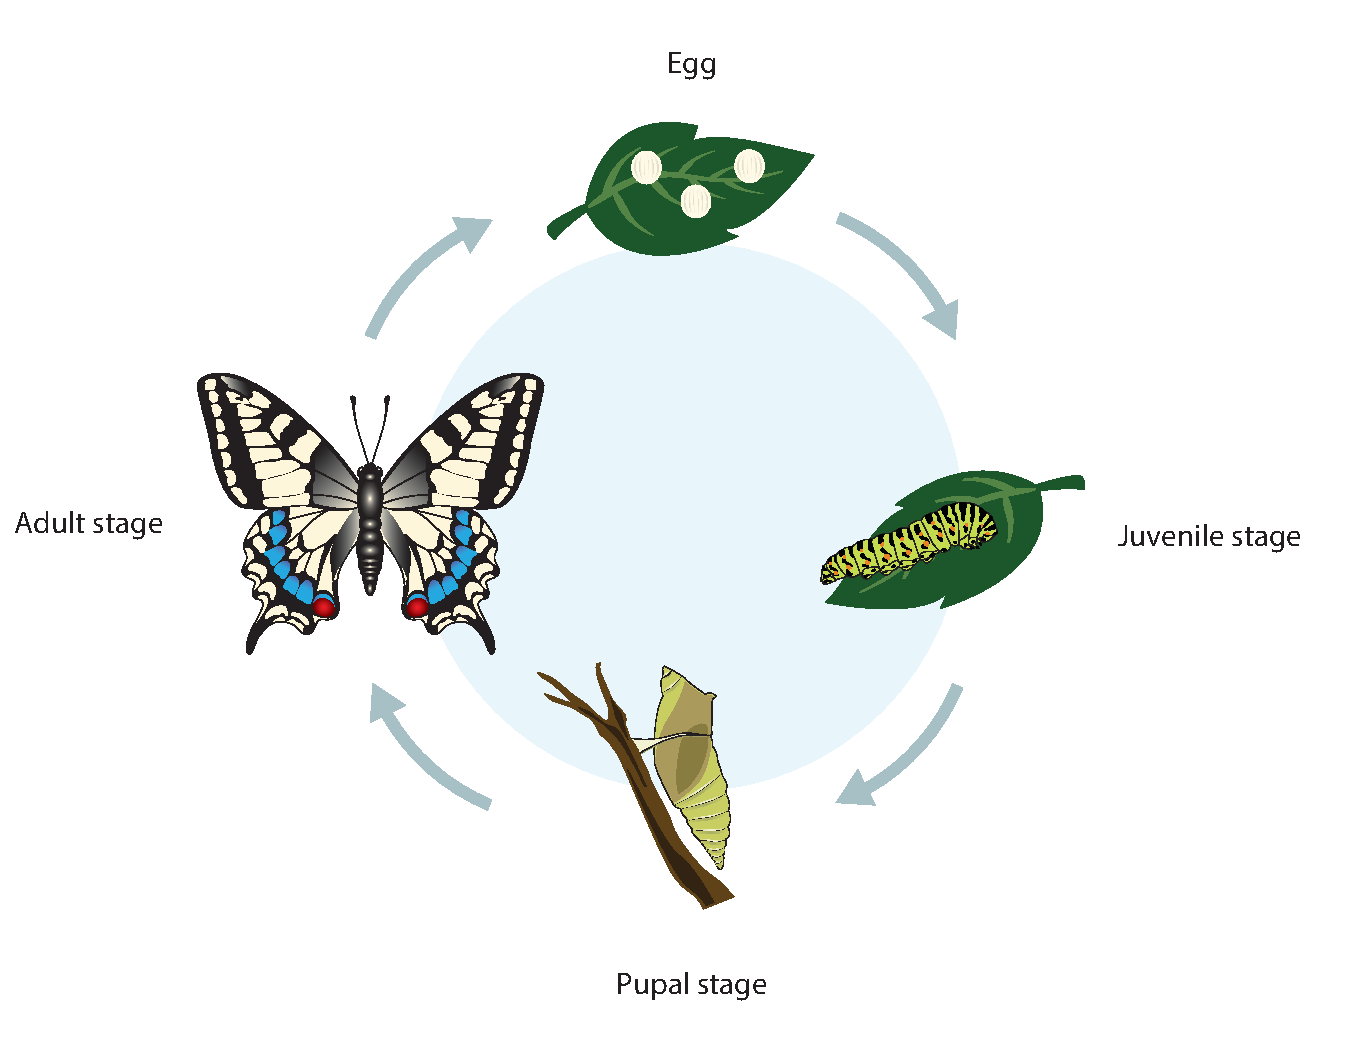
\includegraphics[width=0.9\textwidth]{papilo_machaon_life_cycle.pdf} 
\end{centering}
\end{figure}

The somatic mutation theory of ageing suggests that the gradual accumulation of somatic mutations leads to a decline in cellular function, which ultimately contributes to the ageing process \cite{Szilard1959-ru}. The theory also implies that shorter-lived species will have a higher somatic mutation rate than longer-lived species. Since somatic mutation rate is inversely proportional to the lifespan of species in mammals \cite{Cagan2022-yn}, I initially conjectured that somatic mutation rate would be higher in insects as most insects are short-lived \cite{Promislow2022-en}. I observed that mutation burden of insects was lower than what might have been expected from the somatic mutation theory of ageing and an alternative explanation was required for this observation (The DToL project sequences one sample per species and age of the sample is often not recorded. The calculation of somatic mutation rate requires multiple samples of different ages). 

As a disposable tissue that does not contribute to the germ line lineage, the human placenta has a higher mutation burden and chromosomal aberrations that are absent from the foetus \cite{Coorens2021-ct}. On the other hand, the human spermatogonia has the lowest somatic mutation rate \cite{Rahbari2016-ot}. Similarly, larval tissue in holometabola (a superorder of insects that undergoes complete metamorphosis) is a disposable tissue like the placenta that does not contribute to the development of the adult insect, and hence, larval tissue does not transmit genetic information to the next generation. During embryonic development, imaginal disc precursors separate from embryonic stem cells programmed for differentiation into larval tissue after the blastoderm stage and imaginal discs are set aside for further development into the structures of the adult insect during the pupal stage (An imaginal disc is a single layer of epithelial sheet that consists of 20 to 40 cells) \cite{Wieschaus1976}. Genitalia, for example, are derived from the medial disc in \textit{D. melanogaster} \cite{Bate1993}. Larva and adult insects are, therefore, derived from distinct embryonic lineage, aside from the histoblast cells that develop into the abdomen of the adult insect \cite{Bate1993}. Consequently, somatic mutations that were acquired in the larval stage should be absent in the adult insect and only the somatic mutations that arose during the first few cell divisions of embryonic development should be shared between the two tissues (Fig \ref{figure:lepidoptera-mutation-burden}). For instance, caterpillars, the larvae of butterflies and moths, primarily consume the leaves, stems and flowers of plants and the subsequent accumulation of chlorophyll pigment might be phototoxic to caterpillars. During photosynthesis, the photoexcitation of chlorophyll pigment is channelled to convert light energy into glucose and oxygen. In contrast, unregulated photoexcitation of chlorophyll pigment produces reactive oxygen species \cite{Foyer2018-in}. Hence, C>A somatic mutations associated with DNA damage by reactive oxygen species (SBS18 and SBS36) might the dominant somatic mutational process in caterpillars. 

\begin{figure}[h!]
\caption{Hypothetical changes in mutation burden with life cycle progression}
\label{figure:lepidoptera-mutation-burden}
\begin{centering}
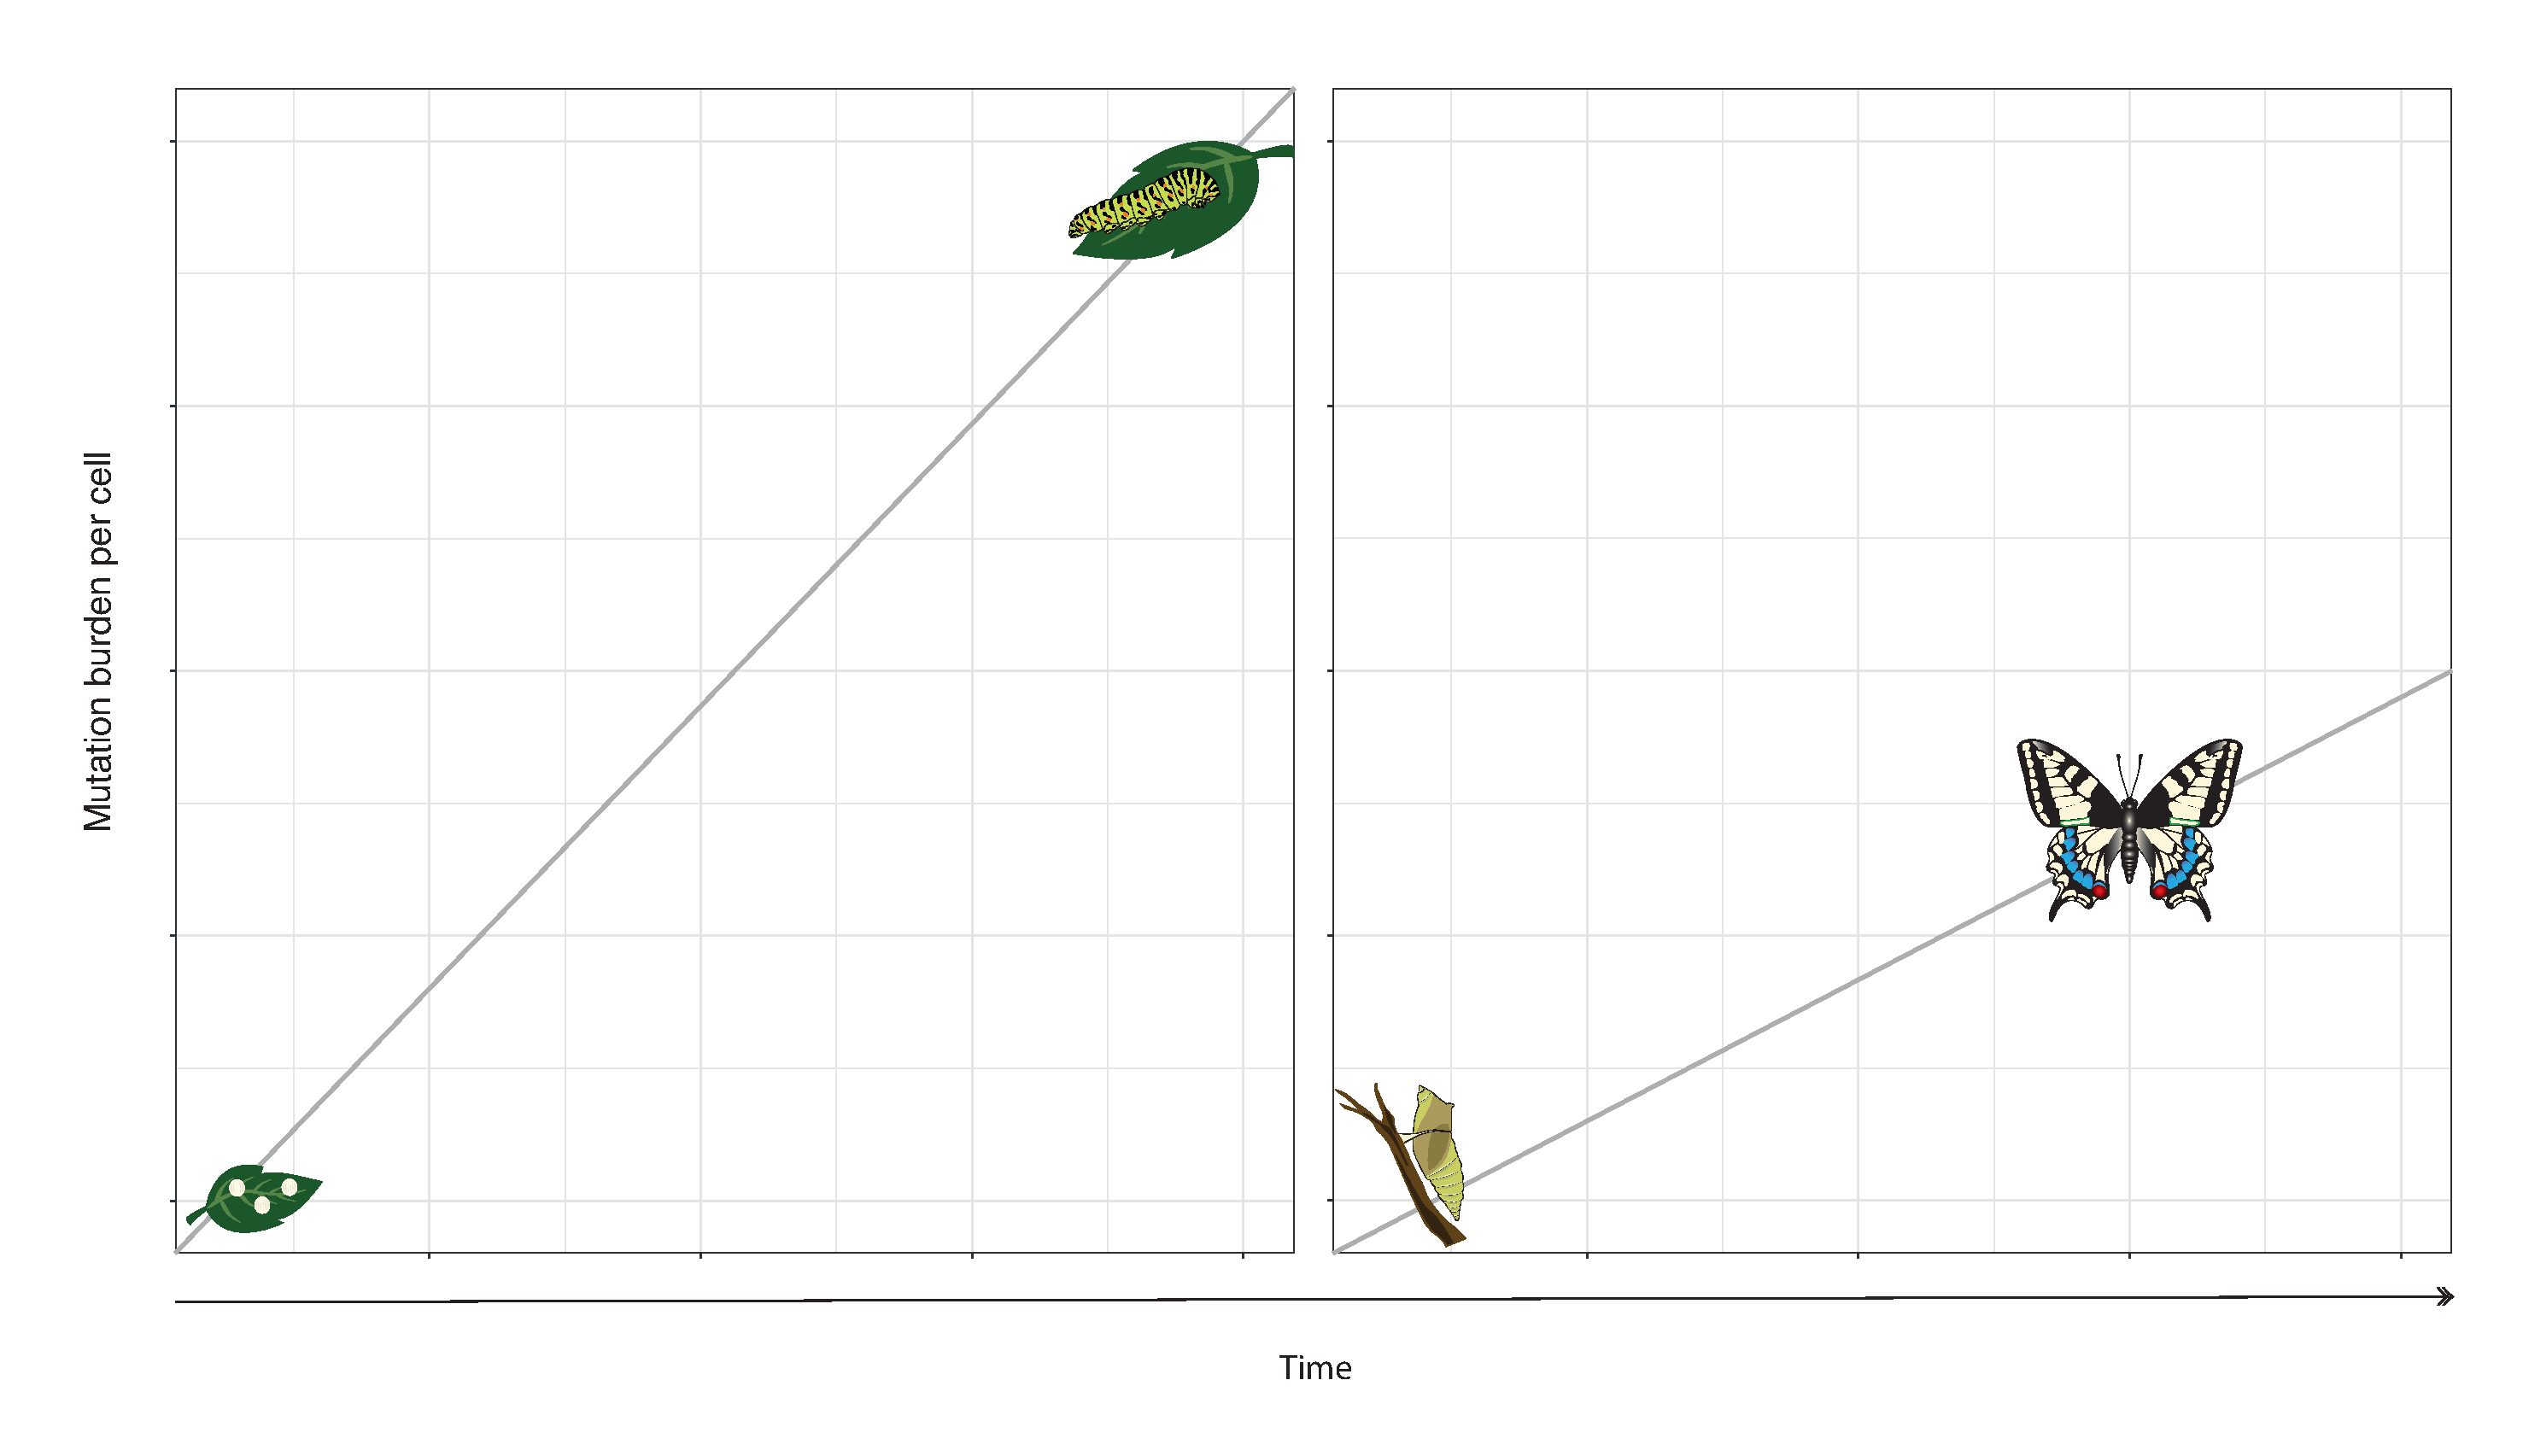
\includegraphics[width=\textwidth]{lepidoptera_mutation_burden.pdf} 
\end{centering}
\floatfoot{Larval tissue is hypothesised to have a higher somatic mutation rate than adult tissue. Somatic mutations acquired during the juvenile stage are not transmitted to the adult insect and a new somatic mutational process is operational in the adult tissue. }
\end{figure}

The life cycle and development of holometabolous insects corroborates the hypothesis that somatic mutations acquired during the larval stage are not shared with the adult insect. In addition, the hypothesis could be tested with insect species that exhibit sexual dimorphism in development. In certain insect species, females do not undergo metamorphosis, referred to as larviform female, while the males still undergo complete metamorphosis. CCS sequencing of both male and female samples with such sexual dimorphism could confirm whether somatic mutation rate is higher in the larval tissue. This experiment, however, does not address the question of why the mutation burden is low in adult insects despite the high cell division rate during metamorphosis. 

\section{Future directions}

In the imminent future, I conjecture that CCS library errors and inaccurate CCS BQ score estimation will be properly addressed and that the majority (>50\%) of CCS bases will have $\sim$Q90 base accuracy. Here, I discuss the potential opportunities following this development.

\subsection{Single-molecule real-time sequencing}

As discussed in chapter 1, CCS sequence throughput and sequencing cost per base is a function of the number of ZMWs and the read-of-insert length of the SMRTbell template. As demonstrated in chapter 2 and chapter 3, CCS base accuracy is a function of subread error rate and the number of subreads per CCS read, under the assumption that there are no new errors introduced during consensus sequence generation. Here, I make some informed predictions about the forthcoming advancements in the SMRT sequencing platform based on observations made in this PhD thesis.

I expect the number of ZMWs per SMRTcell to double every two to three years like how Moore’s Law predicts the number of transistors per chip to double every two years. As the number of ZMWs per SMRTcell increases exponentially, sequencing cost per base is expected to decrease exponentially as well (Fig \ref{figure:ccs_sequence_throughput}a). Moore’s law has continued for approximately $\sim$50 years and similar performance increases can be expected from SMRTcell as well. In addition, as CCS sequence throughput is directly proportional to CCS read length, the rate at which CCS sequence throughput increases could also exceed all our expectations due to the combined effect of parallel increases in both CCS read length and number of ZMWS per SMRTcell (Fig \ref{figure:ccs_sequence_throughput}b). 

\begin{figure}[h]
\caption{Exponential decay in CCS sequencing cost}\label{figure:ccs_sequence_throughput}
\begin{centering}
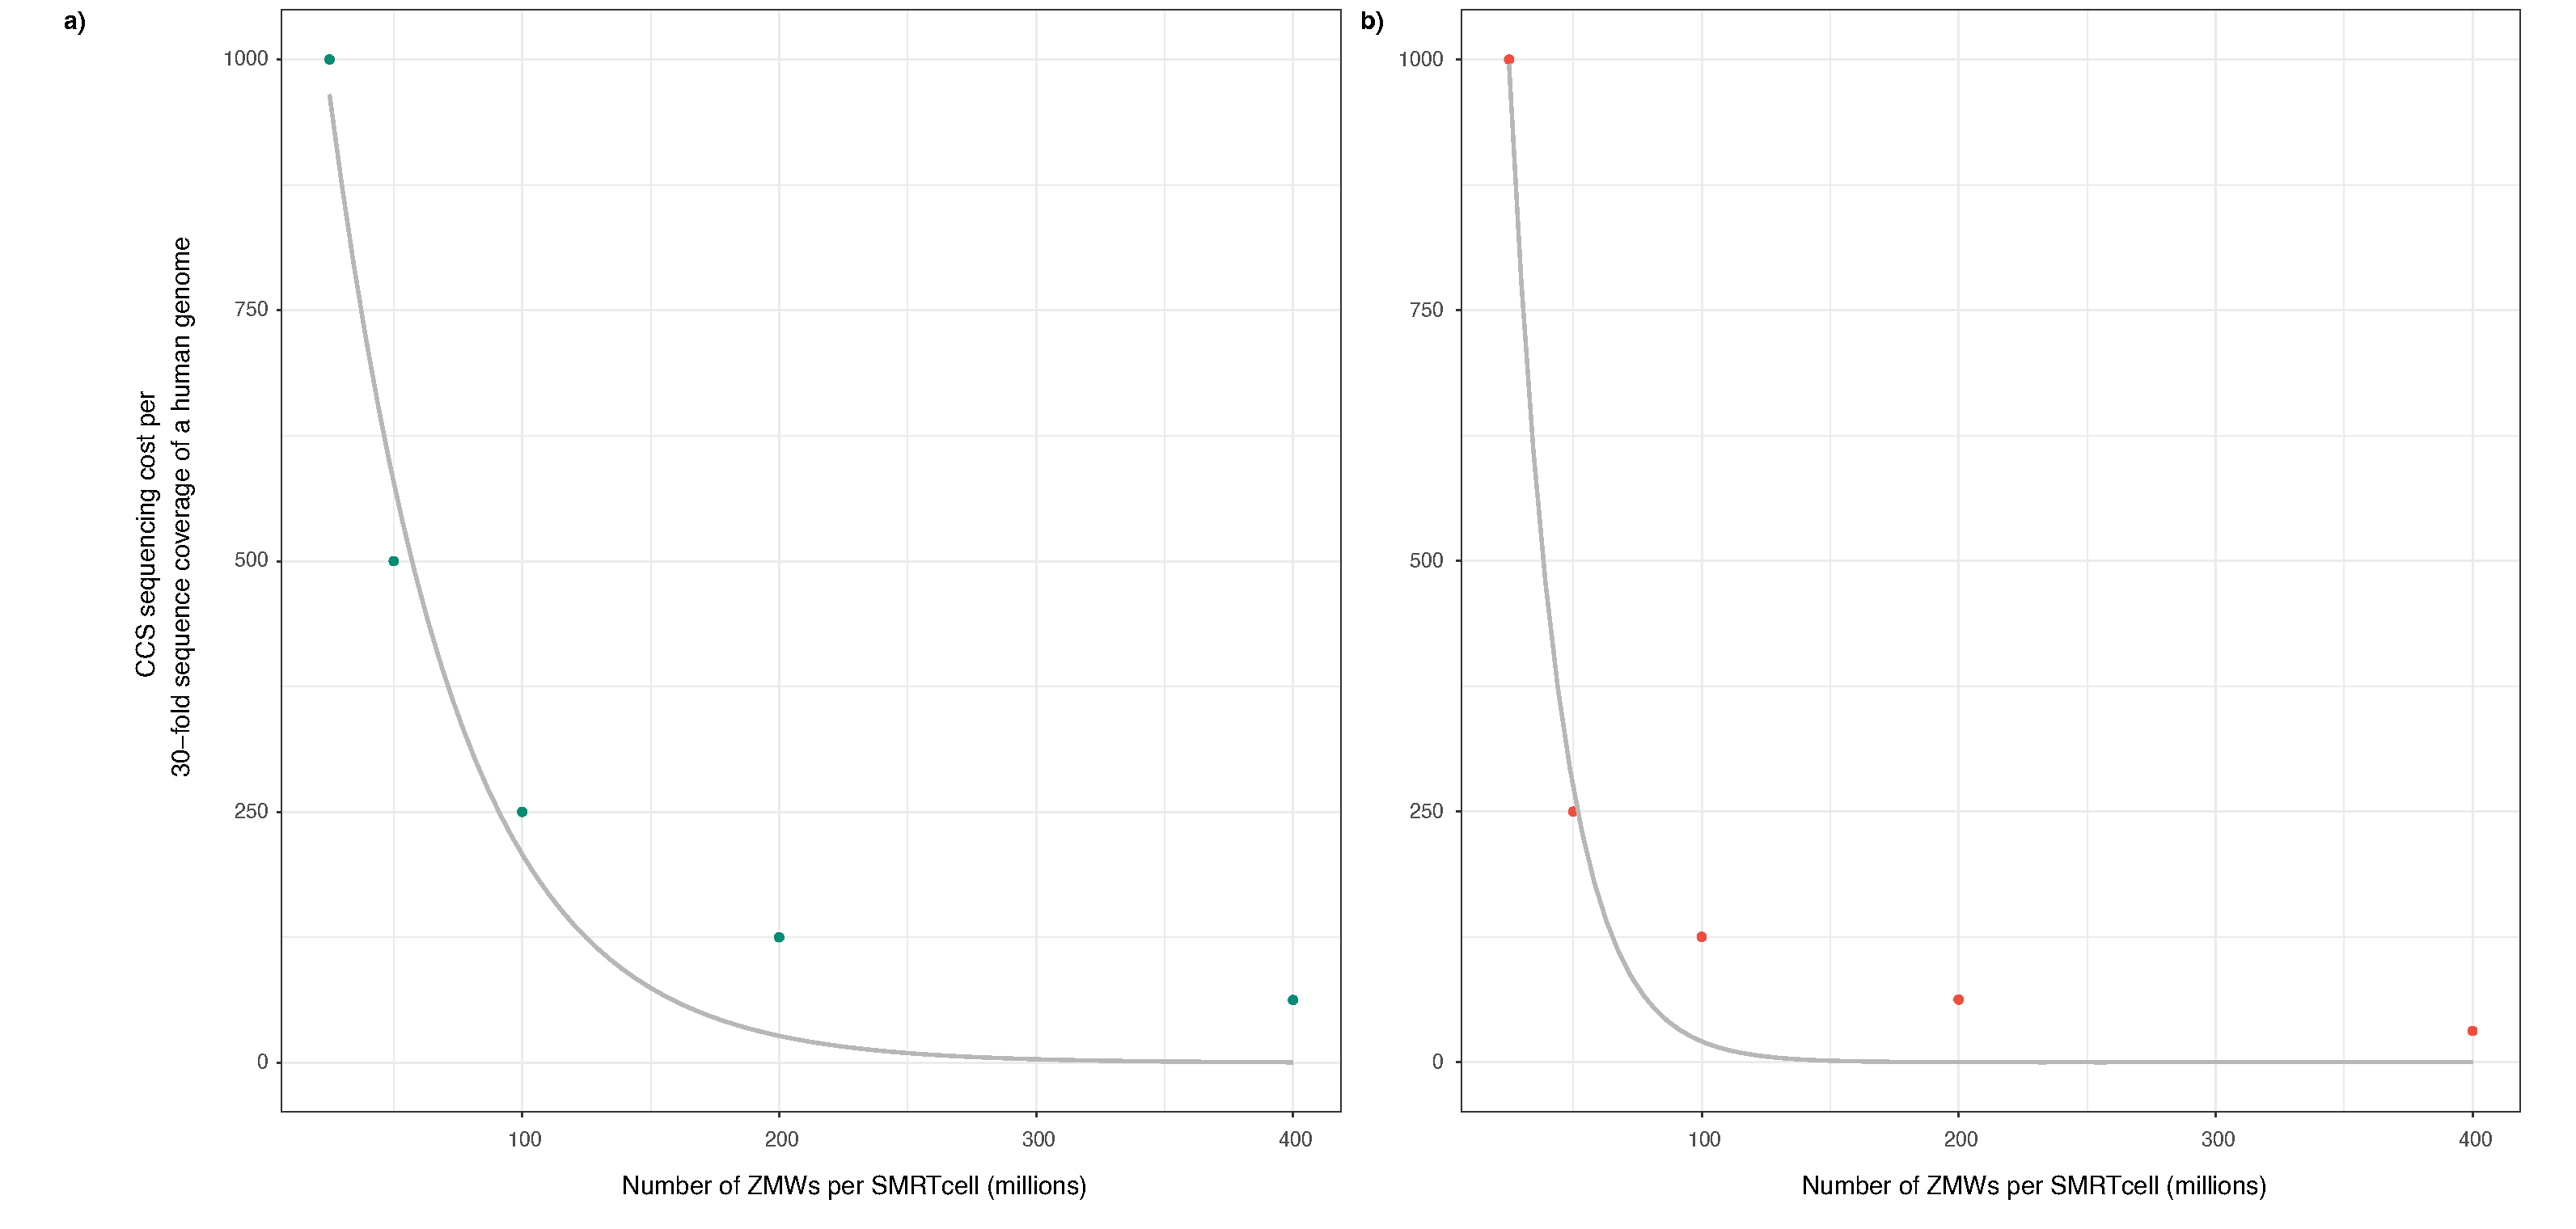
\includegraphics[width=\textwidth]{exponential_decay_in_ccs_sequencing_cost.pdf} \\ \smallskip
\end{centering}
\floatfoot{The graph starts with the current CCS sequencing cost for a 30-fold sequence coverage of a human genome using the Revio instrument, the latest SMRTcell with 25 million ZMWs and assumes that average CCS read length is around 20kb. \textbf{a)} Exponential decay in CCS sequencing cost with doubling in the number of ZMWs per SMRTcell. \textbf{b)} Exponential decay in CCS sequencing cost with doubling in both CCS read length and the number of ZMWs per SMRTcell.}
\end{figure}

To make accurate predictions about future technological advances, I must also consider Wright’s Law, a companion of Moore’s Law. Wright’s Law, also known as experience curve effect, states that for every cumulative doubling of units produced, costs will fall by a constant percentage. As discussed above, the rapid decrease in CCS sequencing costs will accelerate the adoption of CCS sequencing and when economies of scale are achieved, the positive flywheel effect will be unstoppable (Fig \ref{figure:flywheel}). 

\begin{figure}[h!]
\caption{Pacific Biosciences flywheel}
\label{figure:flywheel}
\begin{centering}
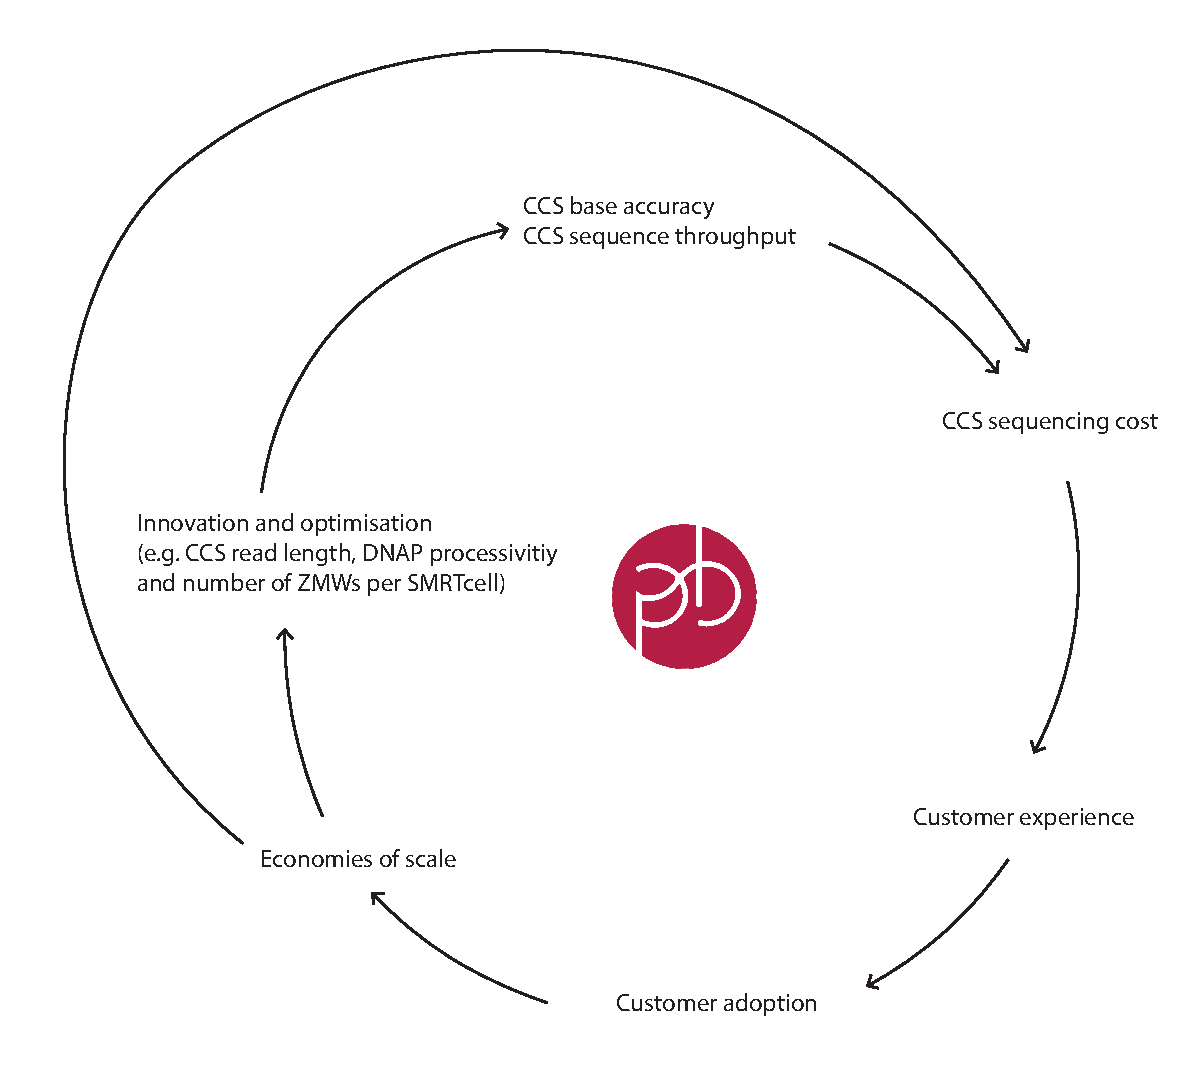
\includegraphics[width=0.75\textwidth]{pacbio_flywheel.pdf} \\ \smallskip
\end{centering}
\floatfoot{The flywheel symbolises how independent components act in concert to improve base accuracy, reduce sequencing cost and drive customer adoption}
\end{figure}


DNAP processivity, the rate at which DNAP synthesises a new strand of DNA, is another crucial factor that determines CCS base accuracy and sequence throughput. If the subread error rate is between 10\% and 15\%, CCS generation typically requires at least 10 subreads per CCS read to generate CCS bases with Q93 base accuracy. DNAP processivity determines the number of subreads per CCS read and hence, increasing DNAP processivity translates to increasing CCS read length. If, for example, DNAP processivity is doubled, CCS read length can also be doubled without sacrifices in base accuracy. DNAP’s biological limit, hence, will be the theoretical limit of CCS read length. In addition, DNAP replication error rate is not an obstacle to $\sim$Q90 CCS base generation at all trinucleotide sequence contexts as demonstrated in chapter 2. One interesting ramification of improved base accuracy is that pooled and non-barcoded samples can be sequenced together to detect common germline SNPs as lower sequence coverage is needed to call the germline mutations with confidence. In addition, as the number of somatic mutations increases linearly with sequence coverage, CCS sequence coverage will not determine the confidence with which germline mutations are detected, but the number of somatic mutations that are detected from the sample. 

In contrast, Illumina’s sequencing by synthesis approach has several disadvantages that limit improvements in read length and base accuracy. In each Illumina sequencing cycle, the rate at which a growing DNA becomes asynchronous with the rest of DNA fragments from the same cluster increases, resulting in a reduced signal-to-noise ratio as sequencing progresses \cite{Metzker2005-am}. This technical limitation places a ceiling on Illumina read length and is responsible for decline in per-base sequence quality towards the end of the read. In addition, CCS sequence throughput is a polynomial function with read length and number of ZMWs per SMRTcell as input while Illumina sequence throughput is a linear function with number of clusters per flow cell as the only input. Consequently, CCS sequencing possesses a greater potential for improving sequence throughput. Considering the fact that CCS reads enables \textit{de novo} assembly and simultaneous detection of haplotype phased somatic and germline mutations and epigenetic modifications, I believe that CCS sequencing will be the primary DNA sequencing method in clinics and research in the imminent future. 

\subsection{Strand-specific somatic mutation detection}

To date, somatic mutation detection in normal tissues and tumours with next-generation sequencing have focused on analysing sub-clonal or clonal somatic mutations that are fixed in a group of cells above the limit of detection threshold. Single-molecule resolution and strand-specific base modification somatic mutation detection has the potential to enhance our understanding of somatic mutagenesis.

As described in chapter 1, DNAP sequences both the forward and reverse strand of the SMRTbell template multiple times through rolling circle replication. The pbccs algorithm leverages the redundancies and complementary base pairing between the forward and reverse strand subreads to generate CCS reads. As demonstrated in chapter 2, CCS reads have sufficient base accuracy for single molecule somatic mutation detection and as described in a previous publication, single-molecule resolution 5mC detection is also possible from CCS DNAP kinetics \cite{Vong2019-bi, Tse2021-or}. The pbccs algorithm can also generate single-strand consensus sequence (SSCS) reads from the forward and reverse strand subreads. Strand-specific somatic mutation and base modification detection with SSCS reads presents an exciting opportunity to analyse somatic mutations from their beginning to their end. 

Somatic mutation is a three-step process: 1) DNA damage, mutation, or modification from endogenous or exogenous sources, 2) failure to detect and repair the DNA damage or mutation, and 3) fixation, persistence of DNA mutation in daughter cells through genetic drift or selection. In a population of DNA molecules, there will be a group of wild type DNA molecules, a group of DNA molecules with DNA damage, mutation or modification, a group of DNA molecules undergoing DNA damage repair and a group of DNA molecules with new somatic mutations (Fig \ref{figure:single-strand-specific-mutation}). 

\begin{figure}[htbp!]
\caption{SBS1 somatic mutational process}
\label{figure:single-strand-specific-mutation}
\begin{centering}
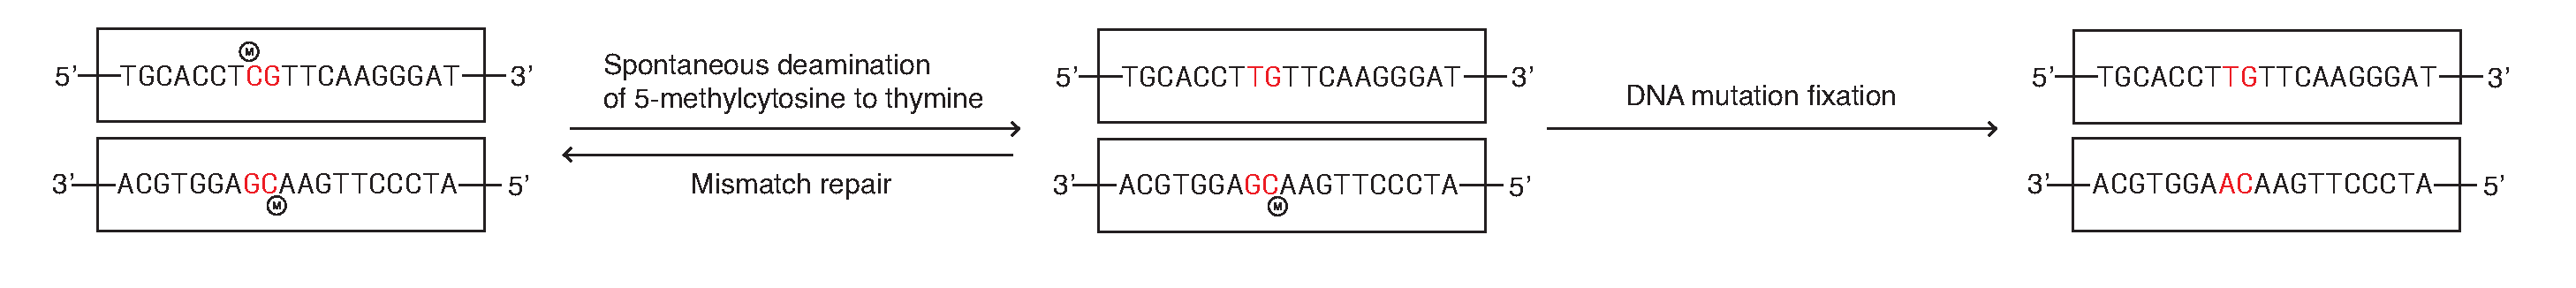
\includegraphics[width=\textwidth]{spontaneous_deamination.pdf} 
\end{centering}
\floatfoot{The figure illustrates how DNA mismatch resulting from spontaneous deamination of 5mC to thymine is repaired and how DNA mutation is fixed. The nucleotide bases in red highlights the methylated CG dinucleotide on both the forward and reverse strand of the DNA.}
\end{figure}

The DNA damage and repair process associated with SBS1 mutational signature, for example, is amenable to further qualitative and quantitative examination through this approach. The spontaneous deamination of 5mC to thymine results in a TG:GC mismatch and results in C>T somatic mutation at a CG dinucleotide if left unrepaired by the mismatch repair (MMR) pathway. If both strands of the double-stranded DNA molecule are sequenced, TG dinucleotide will be present on the strand where deamination has happened and GC dinucleotide with methylation will be present on the complementary strand. SSCS reads from SMRT sequencing enable the detection of TG:GC mismatches and associated hemi-methylation (Figure \ref{figure:single-strand-specific-mutation}). In addition, CCS reads allow the estimation of the number of methylated CG dinucleotides where deamination could have happened and the number of CG dinucleotides where somatic mutations have occurred. If the same tissue is sequenced at multiple different timepoints, the gain and loss of somatic mutations in the population can also be studied.

If successful, we will be able to measure the \textit{in vivo} deamination rate from the number of TG:GC mismatch and the number of GC dinucleotides, and compare it against the \textit{in vitro} deamination rate of $5.8\times10^{-13}$ per 5mC per second at 37°C \cite{Shen1994-of}. In addition, TG:GC mismatch repair efficiency and fidelity can also be measured under wild-type and mutant conditions. MutS$\alpha$, for example, is critical in recognising the TG:GC mismatch and initiating DNA damage repair. MutS$\alpha$ deficiency, therefore, elevates the number of C>T somatic mutations. Similarly, cross-examination of both SSCS and CCS reads and associated DNAP kinetics can also be used to better understand the C>T (SBS2) somatic mutations resulting from APOBEC-dependent deamination of cytosine to uracil.  

\subsection{Decomposition of a mutational signature}

Single-molecule resolution and strand-specific base modification somatic mutation detection, most importantly, creates an opportunity to gain greater insights into the dynamics of somatic mutational processes. Each somatic mutational process leaves a characteristic imprint to the genome and mutational signatures represent the probability that a specific somatic mutational process will produce a somatic mutation in a specific sequence context. Given a catalogue of somatic mutations from multiple samples, mutational signature analysis identifies the mutational signature in each sample and the contribution of each mutational signature to the mutation burden of the sample.

Since each mutational signature is a cumulative result of DNA damage, mutation or modification, failure to repair the DNA damage or mismatch, and persistence of the mutation in bulk tissue, each mutational signature can be re-defined as such (eq. \ref{eq:3})

\begin{align}
\begin{split} 
\alpha D \cdot \beta R \cdot \gamma F &\approx P_{i} \label{eq:3} \\
\alpha \begin{bmatrix}
    d^{1}_{1}  \\
    \vdots &  \\
    d^{96}_{1}  \\
\end{bmatrix} 
\beta \begin{bmatrix}
    r^{1}_{1} \\
    \vdots &  \\
    r^{96}_{1} \\
\end{bmatrix} 
\gamma \begin{bmatrix}
    f^{1}_{1}  \\
    \vdots &  \\
    f^{96}_{1}  \\
\end{bmatrix} &\approx
\begin{bmatrix}
    p^{1}_{1} \\
    \vdots \\
    p^{96}_{1} \\
\end{bmatrix}
\end{split}
\end{align}

where $D$ is the DNA damage matrix and each element is a probability that a specific sequence context will be damaged. $R$ is DNA damage repair matrix and each element is a probability that DNA damage in a specific sequence context will be repaired. $F$ is DNA mutation fixation matrix and each element is a probability that the mutation type will be fixed in the population. $\alpha$, $\beta$, $\gamma$ are scalar values that represent genetic and environmental factors that modulate the somatic mutational process. In addition, $R$ could be further decomposed into multiple subcomponents where each matrix represents a different DNA damage repair pathway specific to the DNA damage (eq. \ref{eq:4})

\begin{equation} \label{eq:4}
\alpha \begin{bmatrix}
    d^{1}_{1}  \\
    \vdots &  \\
    d^{96}_{1}  \\
\end{bmatrix} \
\beta \left[\begin{bmatrix}
    r^{1}_{i} \\
    \vdots &  \\
    r^{96}_{i} \\
\end{bmatrix} 
\begin{bmatrix}
    r^{1}_{i+1} \\
    \vdots &  \\
    r^{96}_{i+1} \\
\end{bmatrix} \ldots 
\begin{bmatrix}
    r^{1}_{n} \\
    \vdots &  \\
    r^{96}_{n} \\
\end{bmatrix}\right]
\gamma \begin{bmatrix}
    f^{1}_{1}  \\
    \vdots &  \\
    f^{96}_{1}  \\
\end{bmatrix} \approx
\begin{bmatrix}
    p^{1}_{1} \\
    \vdots \\
    p^{96}_{1} \\
\end{bmatrix}
\end{equation}

The decomposition of a mutational signature into their individual components and subcomponents should enable us to have a greater understanding of the nonlinear relationship between the components and the mechanisms underlying somatic mutagenesis.

\subsection{Gene conversion and crossover detection}

Here, I also hypothesise that CCS read length and base accuracy can be leveraged to detect gene conversion and crossover events generated during meiotic and mitotic recombination. Gene conversion and crossover (CO) (Fig \ref{figure:homologous-recombination}) arise from the non-reciprocal and reciprocal exchange of genetic material during double-strand break (DSB) repair through homologous recombination. Gene conversions are also referred to as non-crossovers (NCO), but gene conversions and crossovers are not mutually exclusive events \cite{Hunter2015-gk}. 

\begin{figure}[htbp!]
\caption{Gene conversion and crossover}
\label{figure:homologous-recombination}
\begin{centering}
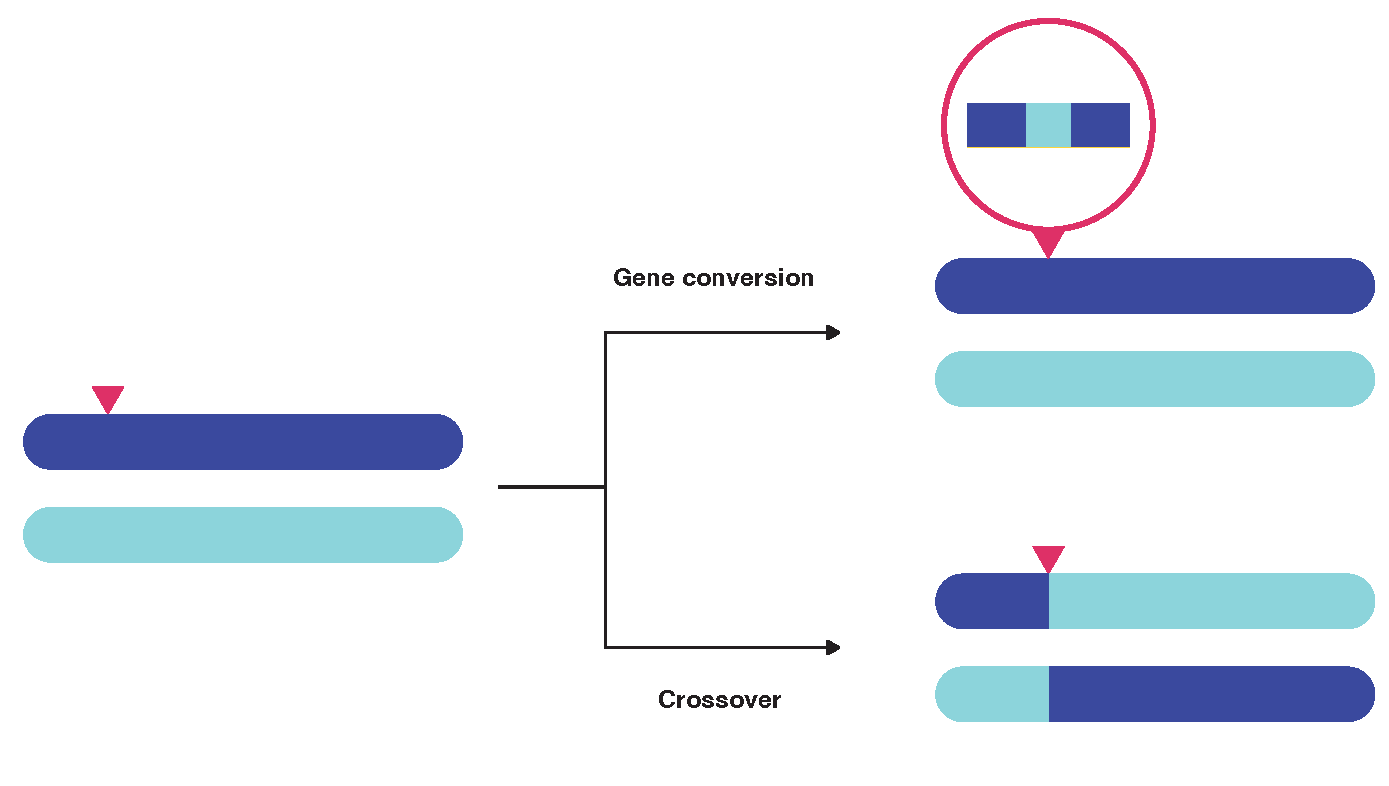
\includegraphics[width=\textwidth]{meiotic_recombination.pdf}
\end{centering}
\floatfoot{Red triangle indicates the DSB site. DSB can be repaired either as a gene conversion or as a crossover. Sister chromatids are not shown for simplification purposes.}
\end{figure}

In germ cells, meiotic recombination is an essential process that generates new combinations of alleles that serve as the foundation for adaptation and speciation through natural selection, an advantage for sexually reproducing organisms. In addition, the formation of at least one chiasma per pair of homologous chromosomes ensures proper segregation of chromosomes in anaphase I of meiosis. Improper chromosome segregation can result in aneuploid gametes with abnormal numbers of chromosomes. If DSB repair is not repaired in somatic cells, DNA damage response initiates programmed cell death. It is worth noting that DSB repair during meiotic recombination generates new allele combinations and contributes to genetic diversity, while DSB repair during mitotic recombination can result in the loss of heterozygosity (LOH). Furthermore, meiotic DSBs are deliberately introduced through the concerted action of PRDM9 and SPO11 to initiate meiotic recombination while mitotic DSBs are inadvertently generated from both endogenous (e.g. reactive oxygen species) and exogenous factors (e.g. ionising radiation).

A haplotype is a set of alleles that are inherited together in a single chromosome. Meiotic recombination yields a new haplotype with a new combination of alleles. Haplotype phasing, therefore, is not only essential for determining the original haplotype before meiotic recombination, but also the haplotype phase switch in individual gametes or in children after meiotic recombination. Trio-sequencing \cite{Kong2010-uk}, sperm-typing \cite{Webb2008-pw} and statistical methods leveraging the non-random association of alleles (linkage disequilibrium) \cite{Myers2005-ml} have been previously used to detect meiotic recombination products and each of these approaches have trade-offs in the resolution and the number of meiotic recombination event detected. Trio-sequencing approach, for example, detects one meiotic recombination per chromosome per child and enables the study of sex-specific meiotic recombination rate. In contrast, sperm-typing of a bulk sperm sample can detect multiple meiotic recombination events per target locus, but it requires prior knowledge of meiotic recombination hotspots. In addition, while statistical methods can generate high-resolution maps of recombination events from patterns of LD in the human population, they are unable to examine meiotic recombination events in an individual.

CCS sequencing of a bulk sperm sample should enable unbiased and genome-wide detection of meiotic recombination events. In addition, the number of detected events should be directly proportional to the sequence coverage as one chiasma per pair of homologous chromosomes is required for physical pairing and proper segregation of chromosomes. If a locus is a meiotic recombination hotspot, CCS sequencing of bulk sperm sample will yield three population of CCS reads: those derived from maternal haplotype, those derived from the paternal haplotype and those resulting from meiotic recombination and containing both maternal and paternal haplotypes. As discussed in chapter 2, CCS read length and base accuracy can be leveraged to phase hetSNPs and connect phased SNPs to construct a haplotype block. CCS haplotype, subsequently, can be determined from comparing CCS hetSNPs to that of the haplotype block. Similarly, CCS reads with both maternal and paternal haplotype can be identified from such a comparison. The length, and the number of phase transitions will also inform whether holliday junction (HJ) was resolved as a gene conversion or a crossover. It is worth noting that the resolution of the recombinant product detection and the number of loci from which recombinant products can be called from is higher in samples with greater heterozygosity. As detailed in chapter 3, many eukaryotic samples have a higher density of SNPs than human samples. In short, CCS base accuracy is used to not detect single molecule somatic mutations but detect single molecule phase transitions (Fig \ref{figure:phase-transitions}).

\begin{figure}[h!]
\caption{Gene conversion and crossover detection using CCS reads}
\label{figure:phase-transitions}
\begin{centering}
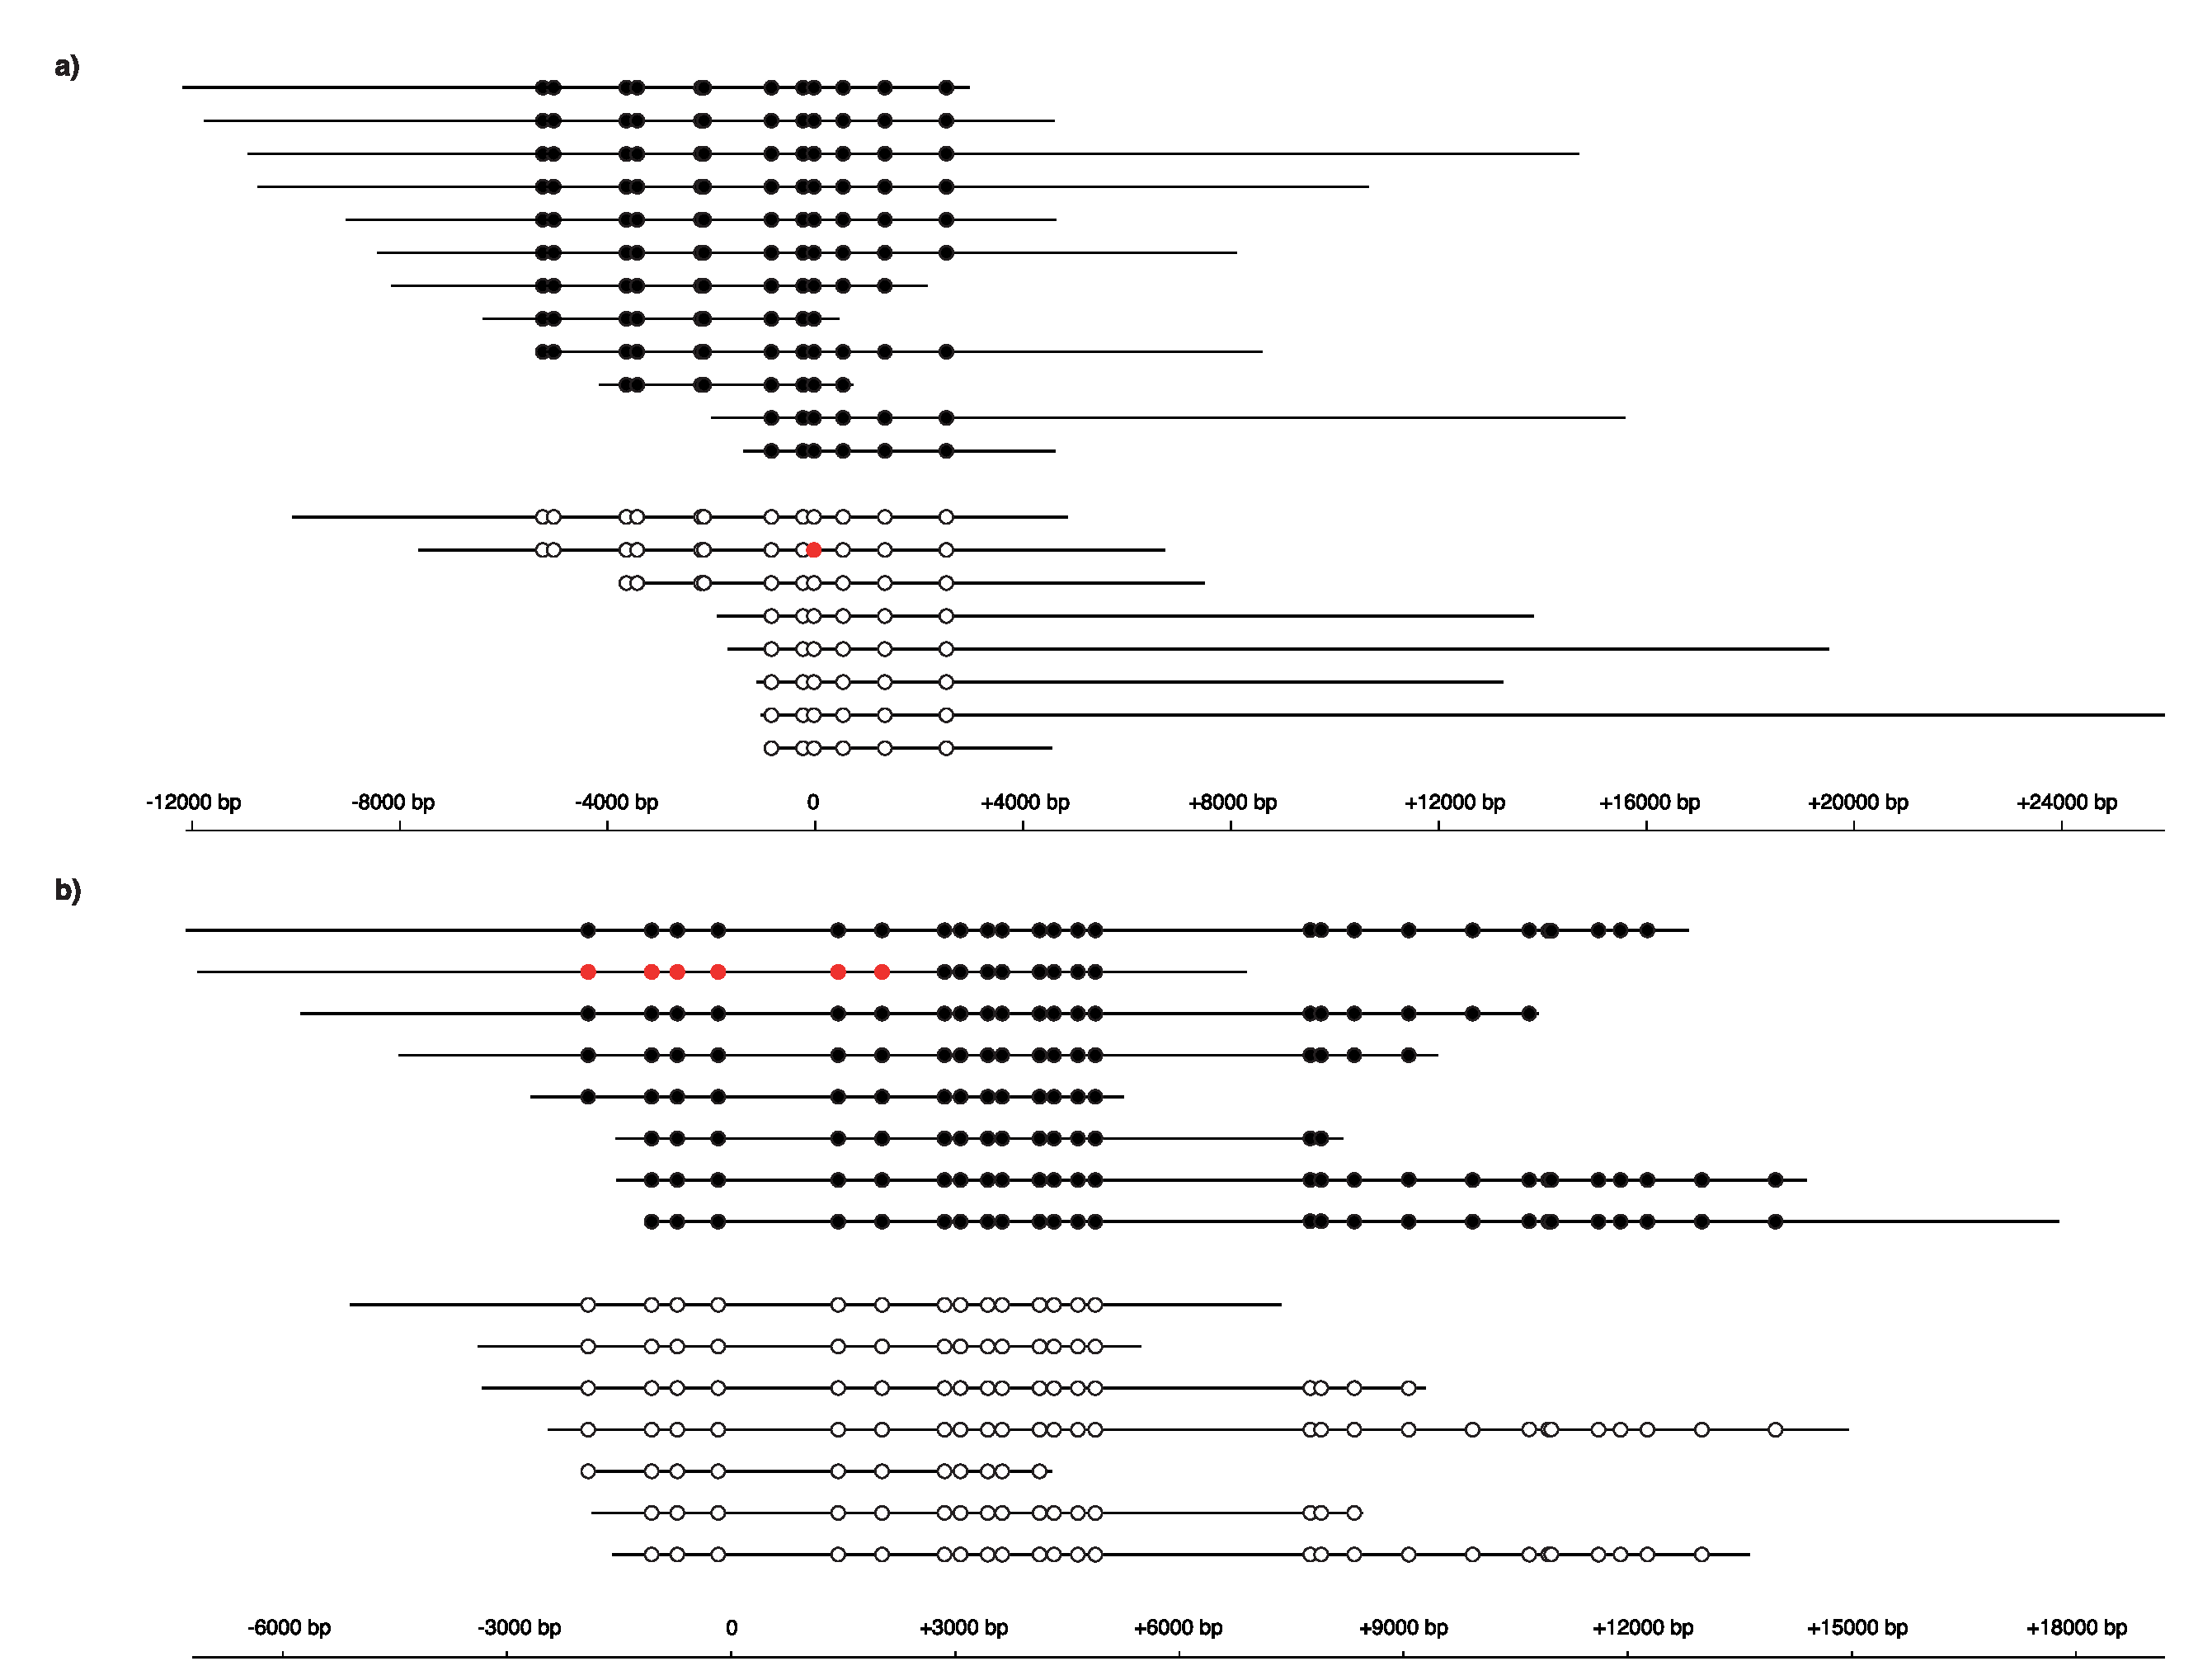
\includegraphics[width=\textwidth]{meiotic_recombination_detection.pdf} 
\end{centering}
\floatfoot{Each circle indicates a heterozygous SNP. A black circle indicates a reference allele, white circle indicates an alternative allele and red circle indicates a phase transition from reference allele to alternative allele and vice versa. CCS reads derived from the same haplotype have the same set of heterozygous SNPs. \textbf{a)} Gene conversion detection using CCS reads requires the phase transition to be flanked by wild type alleles of the haplotype. \textbf{b)} Crossover detection using CCS reads necessitates the phase transition to be continuous.}
\end{figure}

Our approach also has several advantages compared to existing methods and can greatly contribute to the body of research attempting to understand the hotspot conversion paradox \cite{Boulton1997-do}. \textit{De novo} mutations, for example, can be detected using himut and mutation burden across multiple samples of different ages can be used to define the germline mutation rate at scale in species where germline mutation rate is unknown. The hotspot conversion paradox stems from the fact that GC biased gene conversion leads to the loss of PRDM9 recognition sites and meiotic recombination hotspots. PRDM9 gene binds to a specific DNA sequence motif (CCNCCNTNNCCNC) \cite{Myers2008-st} and initiates meiotic recombination through the recruitment of SPO11 for programmed induction of double-strand breaks. The polymorphisms in the zinc finger array determine the exact DNA sequence motif and the PRDM9 binding site. The ability to determine the PRDM9 allele, identify PRDM9 \textit{de novo} mutations and detect gene conversion events using CCS reads should enable us to better understand how the rapid evolution of the PRDM9 gene resolves this paradox. 

The application of the above approach to somatic cells should enable the comprehensive characterisation of mitotic recombination and an assessment of how loss of heterozygosity contributes to oncogenesis in normal cells. Bloom syndrome patients, for example, with an autosomal recessive mutation in the BLM gene have increased risk of developing cancer \cite{Gruber2002-ck}. In addition, cross-examination of both meiotic and mitotic recombination products should elucidate the similarities and differences between these two processes and enhance our understanding of speciation and tumorigenesis. 

\section{Concluding remarks}

I conclude that factors that prevent the adoption of CCS sequencing are technical problems where solutions exist. As discussed in chapter 2, almost error-free CCS bases can be generated and as conjectured in this chapter, CCS sequencing cost and HMW DNA input requirement for CCS library preparation will no longer be a limitation to research. The exponential increase in the number of ZMWs per SMRTcell and the read-of-insert length will be the primary factors driving the increase in sequence throughput and decrease in per-base sequencing cost. The present sequencing methods necessitates a specific DNA input requirement to sequence the genome multiple times and thereby enable the detection of mutations with greater confidence despite the presence of sequencing errors. If DNAP processivity improves to enable CCS library preparation from longer read-of-insert and if CCS base accuracy improves to be error-free, only a single read will be required from each haplotype for germline and somatic mutation detection and epigenetic modification identification, drastically lowering the HMW DNA input requirements for CCS library preparation. I believe that we are witnessing a historic moment where error-free sequencing will be feasible at a fraction of current sequencing costs and where it will be possible to interrogate the genetic, epigenetic, and transcriptomic information of all forms of life.  









